%Turn off page numbering
\pagenumbering{gobble}
\begin{center}

\Huge{Simulations of an impulsive model for the growth of fruit trees}\\
\vspace{\baselineskip}
\LARGE{Theme 08 - Introduction to Systems Biology}\\
\large{Reproduce research}\\
\vspace{\baselineskip}

\begin{figure}
  \centering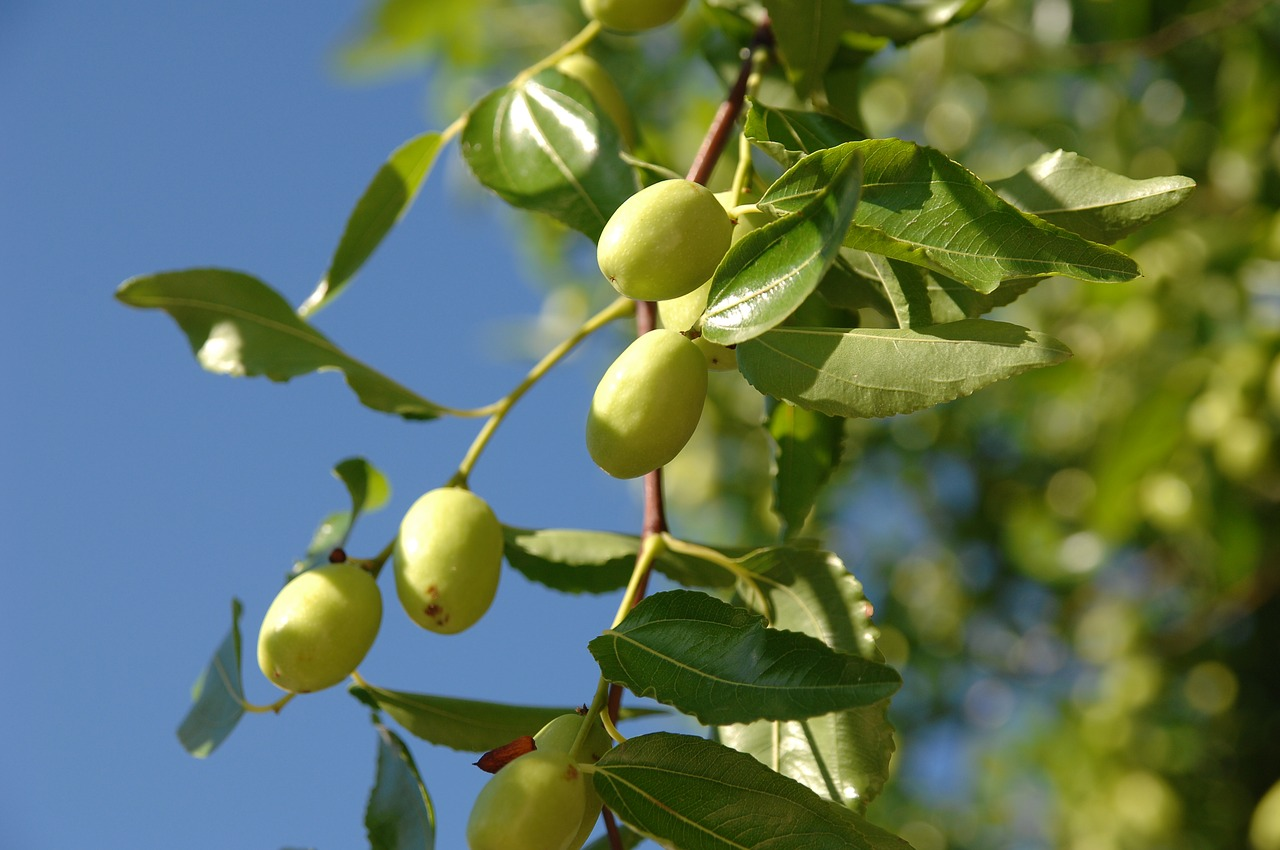
\includegraphics[width=\linewidth]{jujube}
  \label{fig:jujube}
\end{figure}

\end{center}
\vspace{\baselineskip}

%Students info
\normalsize
\vspace*{\fill}
\begin{flushright}
Lisa J.B. Hu (414264)\\
Niek R. Scholten (388602)\\
Bio-Informatics BFV2\\
Institute of Life Science \& Technology\\
Hanze University of Applied Sciences\\
Tsjerk Wassenaar\\
\today
\end{flushright}
\newpage

%Blank page
\null
\thispagestyle{empty}
\addtocounter{page}{-1}
\newpage

\begin{center}

%Titles

\Huge{Simulations of an impulsive model for the growth of fruit trees}\\
\vspace{\baselineskip}
\LARGE{Theme 08 - Introduction to Systems Biology}\\
\vspace{\baselineskip}

\end{center}
\vspace{\baselineskip}

%Students info
\normalsize
\vspace*{\fill}
\begin{flushright}
Lisa J.B. Hu (414264)\\
Niek R. Scholten (388602)\\
Bio-Informatics BFV2\\
Institute of Life Science \& Technology\\
Hanze University of Applied Sciences\\
Tsjerk Wassenaar\\
\today
\end{flushright}
\newpage

\pagenumbering{roman}
\section*{Abstract}

Droughts have affected the agriculture in the mediterranean in an increasingly severe matter.
The decrease in rainfall and the effects of global warming have taken their toll on many orchards, especially fruit producing ones.
Since the water supply of these orchards is always artificial because of the aforementioned factors, dwindling water capacities in reservoirs is a serious issue.
This study aims to provide an insight into the effects of different irrigation patterns on the growth of these fruit trees.
Without a sustainable plan for irrigation, whole populations of fruit trees might perish under a critical water deficit.

\label{sec:abstract}~\addcontentsline{toc}{section}{\nameref{sec:abstract}}
\newpage

\section*{Summary}
Climate change is one of the most severe problems facing planet earth right now.
As a result of this, increasingly crippling droughts have swept over the mediterranean.
This study is based on research of the jujube tree and the growth of its fruit under different irrigation circumstances.
The main issue is the amount of work required to test this growth under varying conditions, so this paper tries to simplify the workflow for researching these scenarios using differential equations.
These models result in vital information for growing patterns, as to better understand the effects of irrigation.
An expansion on these models was also made to incorporate day and night cycles, this proved fruitful as the results drastically changed.
The models were run using the deSolve package for R, and visualised using ggplot2.

\label{sec:summ}~\addcontentsline{toc}{section}{\nameref{sec:summ}}
\newpage

\section*{List of Abbreviations}

\textbf{ODE} Ordinary Differential Equation

\label{sec:abvs}~\addcontentsline{toc}{section}{\nameref{sec:abvs}}

\newpage